\documentclass{article}
\usepackage{graphicx} % Required for inserting images
\usepackage{tabularx} % Agregar esto en el preámbulo
\usepackage{float}  % Permite el uso de [H] para fijar las imágenes en su lugar

\begin{document}

	%%%%%%%%%%%%%%%%%%%%%%%%%%%%%%%%%%%%%%%%%%%%%%%%%%%%%%%%%%%%%%%%%%%%%%%%
	\chapter{Técnicas de Optimización Geoespacial usando Datos del Censo}
	\textbf{Autor}: \large{Cristhian Arlindo Mamani Nina}
	\label{chap:9}
	
	\vspace{1cm} 
	
\section*{9.1 Estructuras de Datos Espaciales y Sistemas de Coordenadas}

\subsection*{Los Datos Espaciales}
Los datos espaciales representan objetos del mundo real en un sistema de coordenadas georreferenciado. Estos datos se pueden clasificar en dos tipos principales:

\begin{itemize}
	\setlength{\itemsep}{-0pt}  % Esto elimina el espacio extra entre los ítems de la lista
	\setlength{\leftmargini}{0pt}  % Esto elimina la sangría a la izquierda
	\item \textbf{Datos vectoriales}: Representan entidades mediante puntos, líneas o polígonos.
	\begin{itemize}
		\setlength{\leftmargini}{1em} % Ajustamos la indentación para las sublistas
		\item \textbf{¿Qué son los Datos Vectoriales?}: Los datos vectoriales representan entidades geográficas mediante tres tipos principales de geometrías:
		\begin{itemize}
			\setlength{\leftmargini}{2em} % Ajustamos aún más la indentación para las sub-sublistas
			\item \small \textbf{Puntos}: Representan ubicaciones específicas, como una estación de tren o un hospital.
			\item \textbf{Líneas}: Representan elementos lineales como carreteras, ríos o redes de transporte.
			\item \textbf{Polígonos}: Representan áreas cerradas como parques, ciudades o regiones administrativas.
		\end{itemize}
		
		\item \textbf{Ejemplo }: Supongamos que tenemos una ciudad con tres elementos geográficos:
		\begin{itemize}
			\item Una estación de tren (\textbf{punto}).
			\item Una carretera (\textbf{línea}).
			\item Un parque (\textbf{polígono}).
		\end{itemize}
		
		Los datos pueden representarse en formato tabular como un archivo CSV:
		\begin{verbatim}
			ID, Tipo, Latitud, Longitud
			1, Punto, -12.0464, -77.0293
			2, Línea, -12.0470, -77.0299
			3, Polígono, -12.0458, -77.0301
		\end{verbatim}
		
		\item \textbf{Procesamiento en SIG}: 
		\begin{itemize}
			\item Se carga el archivo CSV en un SIG como QGIS o ArcGIS.
			\item Se georreferencian los puntos en el mapa.
			\item Se visualizan los elementos y se pueden calcular distancias, áreas o intersecciones.
		\end{itemize}
		
		\item \textbf{Figura}: 
		\begin{figure}[H]
			\centering
			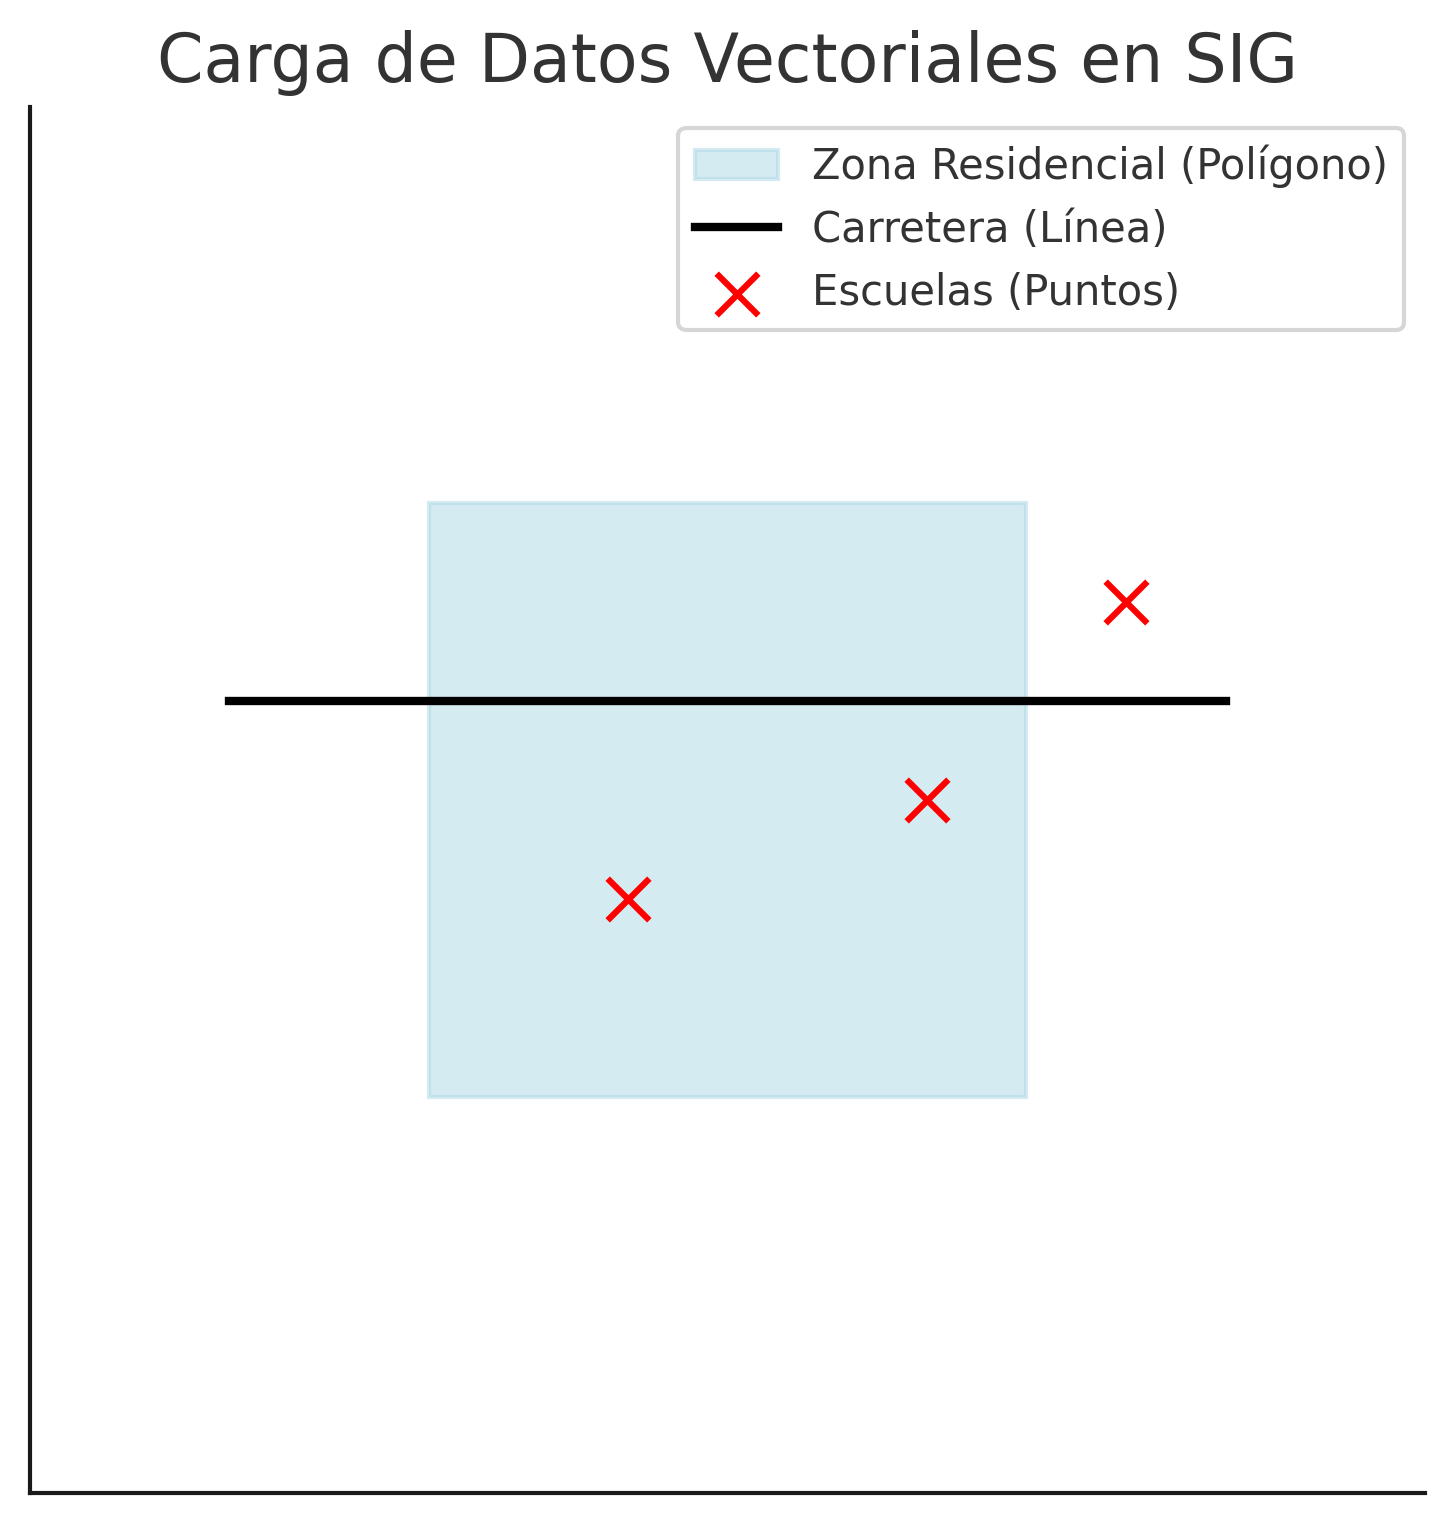
\includegraphics[width=0.5\textwidth]{vec1.png}
			\caption{Ejemplo de representación de datos vectoriales en un SIG.}
		\end{figure}
	\end{itemize}
	
	
	
	
	\item \textbf{Datos Raster}: Los datos raster representan la información espacial mediante una cuadrícula de píxeles. Cada celda de la matriz contiene un valor que representa una característica del terreno.
	\begin{itemize}
		
		\item \textbf{Ejemplo }: Un ejemplo típico de datos raster es un mapa de temperatura donde cada píxel representa una temperatura en una región.
	\end{itemize}
	
	% La tabla debe estar fuera del entorno itemize
	\begin{table}[ht]
		\centering
		\caption{Ejemplo de Datos Raster (Mapa de Temperatura)}
		\begin{tabular}{|c|c|c|}
			\hline
			Píxel X & Píxel Y & Temperatura (°C) \\
			\hline
			1 & 1 & 20 \\
			1 & 2 & 21 \\
			2 & 1 & 22 \\
			2 & 2 & 23 \\
			\hline
		\end{tabular}
	\end{table}
	
	\begin{itemize}
		\item \textbf{Procesamiento en SIG}:
		\begin{itemize}
			\item Se carga el archivo raster (GeoTIFF, PNG con georreferenciación, etc.).
			\item Se visualizan los valores de cada píxel en el mapa.
			\item Se realizan análisis espaciales como interpolaciones o detección de cambios.
		\end{itemize}
	\end{itemize}
	
	% La figura también debe estar fuera del entorno itemize
	\begin{figure}[ht]
		\centering
		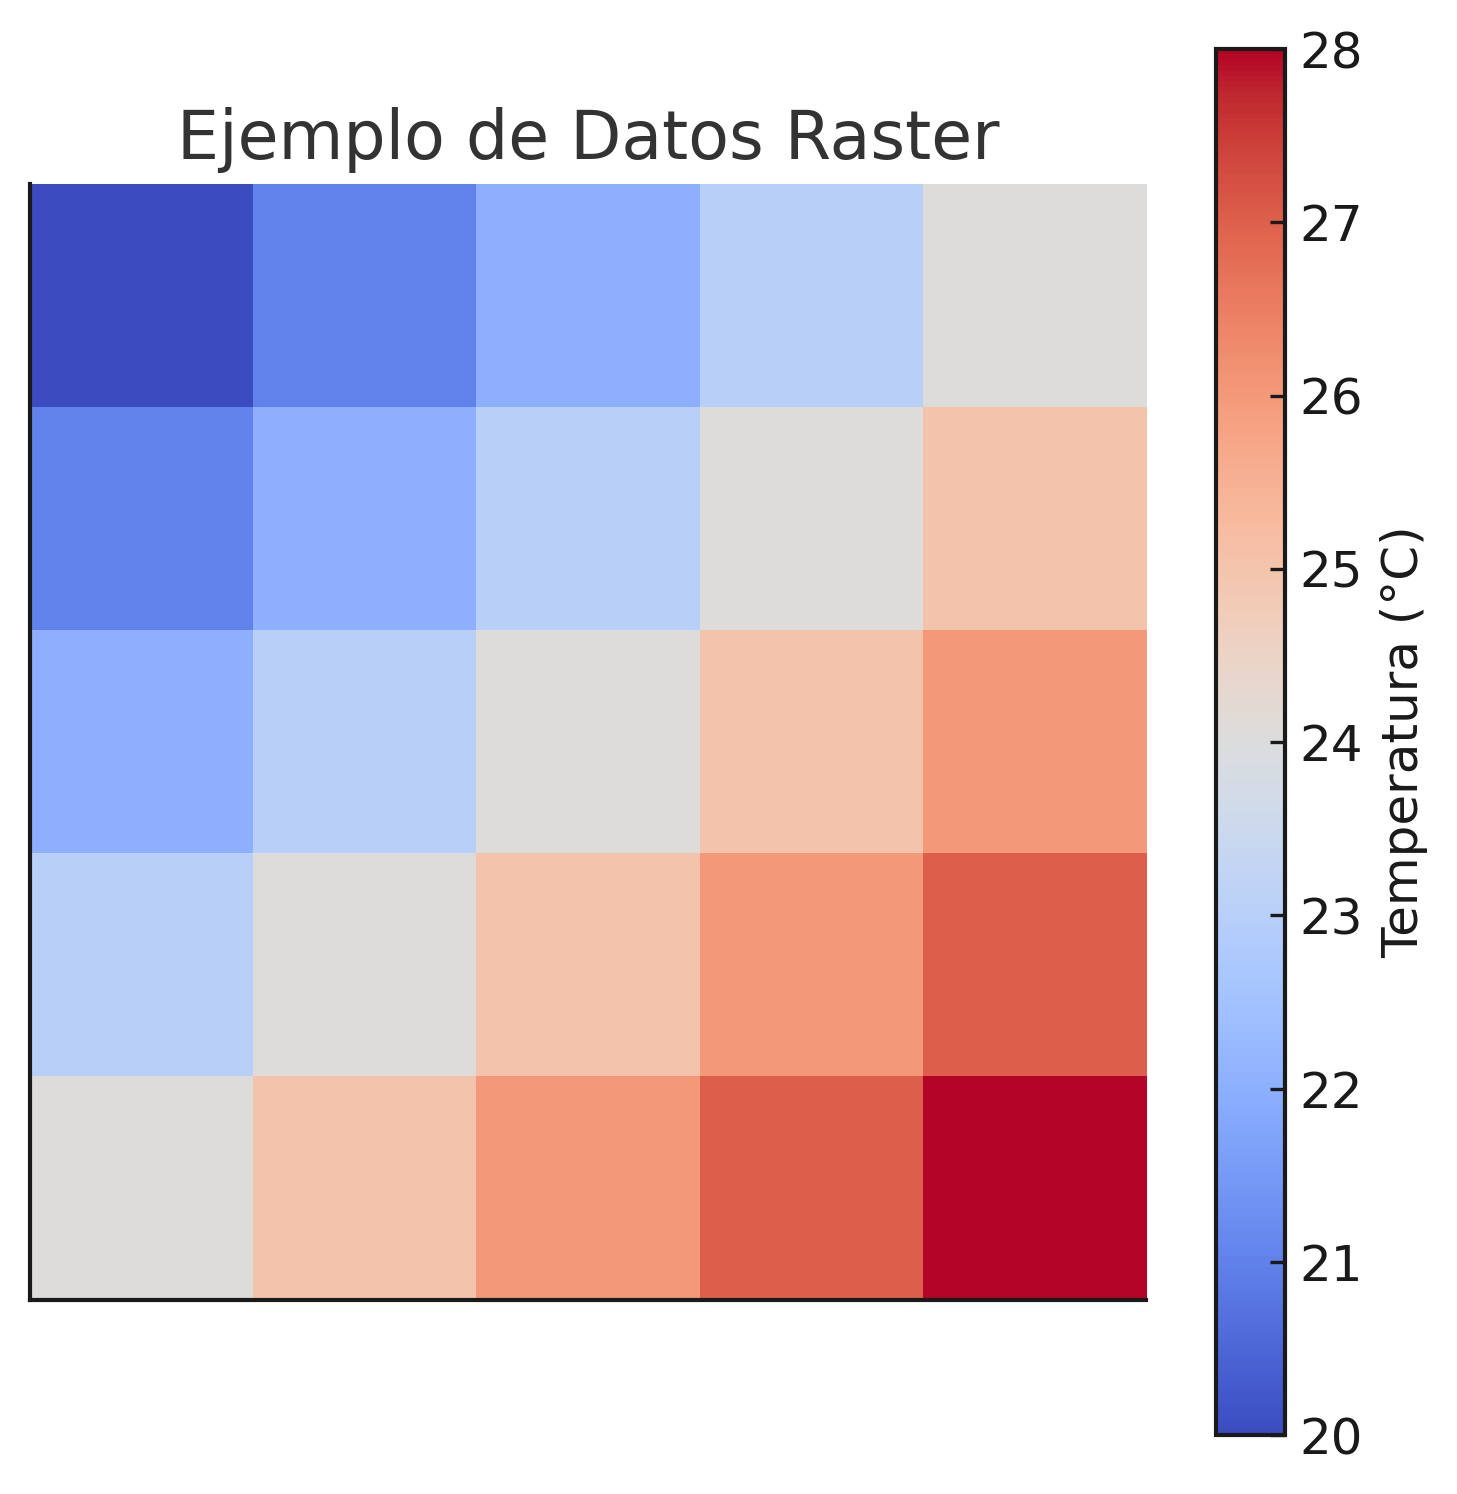
\includegraphics[width=0.6\textwidth]{ras1.png}
		\caption{Ejemplo de representación de datos raster en un SIG.}
	\end{figure}
	
	
	
	
	El \textit{Directorio Nacional de Centros Poblados 2023} del INEI está organizado en formato tabular (CSV), pero cada registro debería estar asociado a una ubicación geográfica con coordenadas para su representación en un SIG (Sistema de Información Geográfica).
	
	\subsection*{Sistemas de Coordenadas y Proyecciones Cartográficas}
	Para representar correctamente los datos espaciales, se utilizan sistemas de coordenadas y proyecciones cartográficas que permiten definir ubicaciones en la Tierra.
	
	\textbf{Tipos de sistemas de coordenadas}:
	\begin{itemize}
		\item \textbf{Geográficos (GCS - Geographic Coordinate System)}: Utilizan latitud y longitud en grados.
		\item \textbf{Proyectados (PCS - Projected Coordinate System)}: Transforman la superficie curva de la Tierra en un plano usando metros o kilómetros.
	\end{itemize}
	
	\textbf{Sistema de coordenadas usado en Perú}:  
	El INEI y la cartografía oficial del Perú utilizan el sistema de referencia global \textbf{WGS 84 (EPSG:4326)} y las proyecciones \textbf{UTM Zona 17S y 18S} para representación precisa en mapas.
	
	\subsection*{Estructura del Directorio Nacional de Centros Poblados 2023}
	El dataset del INEI proporciona información clave sobre los centros poblados en Perú. Algunas columnas relevantes incluyen:
	
	\begin{table}[H]
		\centering
		\renewcommand{\arraystretch}{1.5}
		\begin{tabularx}{\textwidth}{|l|X|}
			\hline
			\textbf{Categoría} & \textbf{Descripción} \\
			\hline
			Ubicación administrativa & Departamento, Provincia, Distrito, Nombre del Centro Poblado. \\
			\hline
			Datos de la autoridad local & Nombre del alcalde, teléfono, correo electrónico. \\
			\hline
			Código único del centro poblado (CCPP) & Identificador que permite cruzar información con otras bases de datos. \\
			\hline
		\end{tabularx}
		\caption{Información estructurada del Centro Poblado}
		\label{tabla:centro_poblado}
	\end{table}
	
	
	\textbf{Desafío}:  
	El dataset no incluye coordenadas geográficas (\textit{latitud, longitud}), por lo que es necesario realizar un proceso de geocodificación para poder mapear la información en un SIG.
	
	\subsection*{Preparación de Datos para su Uso en QGIS, ArcGIS y GeoPandas}
	Para trabajar con este dataset en herramientas SIG, se deben seguir los siguientes pasos:
	
	\begin{itemize}
		\item \textbf{Cargar el archivo CSV en QGIS o ArcGIS}. Si no tiene coordenadas, se puede unir con otra fuente que las contenga.
		\item \textbf{Estandarizar los datos y asignar un sistema de coordenadas}. Convertir códigos administrativos en ubicaciones geoespaciales.
		\item \textbf{Generar visualizaciones iniciales} para validar la distribución de centros poblados.
	\end{itemize}
	
	\textbf{Ejemplo práctico}:  
	Si se encuentra un dataset complementario con coordenadas, se puede hacer una \textit{unión de datos} en GIS para georreferenciar la información del INEI.
	
	\section*{9.2 Problemas de Ubicación de Instalaciones y Optimización de Cobertura}
	
	\subsection*{Los Modelos de Optimización}
	En planificación territorial y distribución de recursos, es fundamental ubicar estratégicamente infraestructuras como hospitales, colegios o estaciones de transporte público. Para ello, se emplean modelos matemáticos que optimizan la cobertura y accesibilidad de estos servicios.
	
	Algunos de los modelos más utilizados incluyen:
	
	\begin{itemize}
		\item \textbf{Modelo de Cobertura Máxima} (Max Covering Location Problem - MCLP): Busca ubicar una cantidad determinada de instalaciones para maximizar la cobertura de la población en un radio definido.
		\item \textbf{Problema del Centro de Mediana} (p-Median Problem): Minimiza la distancia promedio entre la población y las instalaciones asignadas.
		\item \textbf{Diagramas de Voronoi}: Técnica geométrica que divide un espacio en regiones de influencia en función de un conjunto de puntos de referencia.
		\item \textbf{Optimización de Rutas}: Algoritmos como \textbf{Dijkstra} o \textbf{A*} ayudan a encontrar los caminos más cortos para la movilidad dentro de un sistema de transporte.
	\end{itemize}
	
	Estos modelos permiten resolver problemas reales, como mejorar el acceso a la salud en áreas rurales, optimizar el transporte público en ciudades o distribuir centros de abastecimiento estratégicamente.
	
	\subsection*{Aplicación del Modelo de Cobertura Máxima}
	El modelo de cobertura máxima (MCLP) es una técnica de optimización que permite ubicar instalaciones (como hospitales) para maximizar la cobertura de la población dentro de un radio determinado. A continuación, se describe su aplicación en el contexto peruano.
	
	
	\begin{table}[H]
		\centering
		\caption{Pasos para Aplicar el Modelo de Cobertura Máxima}
		\begin{tabularx}{\textwidth}{|l|X|}
			\hline
			\textbf{Paso} & \textbf{Descripción} \\
			\hline
			1. Definir datos de entrada & Utilizar el \textit{Directorio Nacional de Centros Poblados 2023} para obtener ubicaciones de centros poblados. \\
			\hline
			2. Establecer radio de cobertura & Definir un radio de 10 km para la cobertura de hospitales. \\
			\hline
			3. Aplicar algoritmo de cobertura máxima & Seleccionar ubicaciones que maximicen la población cubierta dentro del radio. \\
			\hline
			4. Visualización en GIS & Generar mapas en QGIS o ArcGIS para analizar las áreas de cobertura. \\
			\hline
		\end{tabularx}
		\label{tab:mclp_pasos}
	\end{table}
	
	\subsection*{Diagramas de Voronoi para la Optimización}
	
	Es una partición de un espacio en regiones basadas en la proximidad a un conjunto de puntos dados. Cada punto en el espacio pertenece a la región cuyo punto de referencia es el más cercano. Este tipo de diagrama es utilizado principalmente en \textbf{geoespacial} para optimizar la ubicación de instalaciones, como hospitales, estaciones de policía o centros comerciales, al dividir un área en zonas de influencia.
\end{itemize}

\subsection*{\small Principio Básico:}

{Dado un conjunto de \textbf{puntos de referencia} (como hospitales), el Diagrama de Voronoi divide el espacio en \textbf{regiones} donde cada región contiene los puntos más cercanos a ese punto de referencia. Es útil para visualizar la cobertura geográfica y la distribución de recursos o servicios.
	
\subsection*{\small Aplicaciones Comunes:}
\begin{itemize}
	\item \small \textbf{Optimización de la ubicación de instalaciones}: Ubicación de hospitales, estaciones de policía, escuelas, etc.
	\item \small \textbf{Análisis de accesibilidad}: Determinar qué áreas están más cerca de un servicio o instalación.
	\item \small \textbf{Distribución de recursos}: Asegurar que las instalaciones cubran de manera eficiente el área de servicio.
\end{itemize}


Por ejemplo, si se tienen 10 hospitales en una ciudad, cada hospital atenderá a la población más cercana a él. Las celdas de Voronoi ayudarán a definir estas áreas de influencia y mejorar la asignación de pacientes.

\begin{figure}[H]  % Aquí H asegura que la imagen se ubique exactamente donde está en el código
	\centering
	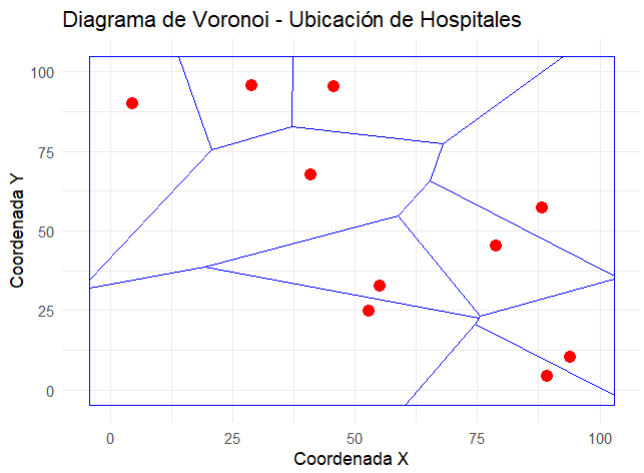
\includegraphics[width=0.7\textwidth]{op.png}  % Cambia "op.png" con el nombre de tu imagen
	\caption{Ejemplo de Diagrama de Voronoi para la distribución de hospitales}
	\label{fig:voronoi}
\end{figure}

\subsection*{\small Código en R }

\begin{lstlisting}
	# Instalar e importar los paquetes necesarios
	install.packages("deldir")
	install.packages("ggplot2")
	
	library(deldir)
	library(ggplot2)
	
	# Generar puntos aleatorios (ubicaciones de hospitales)
	set.seed(42)
	points <- data.frame(
	x = runif(10, min = 0, max = 100),  # 10 puntos aleatorios para las X
	y = runif(10, min = 0, max = 100)   # 10 puntos aleatorios para las Y
	)
	
	# Calcular el diagrama de Voronoi
	voronoi <- deldir(points$x, points$y)
	
	# Graficar el diagrama de Voronoi
	ggplot() +
	geom_tile(data = voronoi$dirsgs, aes(x = x, y = y, fill = factor(group)), color = "blue", alpha = 0.3) +
	geom_point(data = points, aes(x = x, y = y), color = "red", size = 4) +
	labs(title = "Diagrama de Voronoi - Ubicación de Hospitales", 
	x = "Coordenada X", y = "Coordenada Y") +
	theme_minimal()
	
	# Guardar el gráfico en un archivo
	ggsave("diagrama_voronoi.png")
\end{lstlisting}

\subsection*{Optimización de Transporte y Movilidad}
El acceso a la infraestructura también depende de la movilidad. Para esto, se pueden aplicar algoritmos de optimización de rutas:

\begin{itemize}
	\item \textbf{Dijkstra}: Encuentra la ruta más corta en una red de caminos (útil para planificación de transporte público).
	\begin{lstlisting}[language=Python]
		import heapq
		
		def dijkstra(graph, start):
		distances = {node: float('inf') for node in graph}
		distances[start] = 0
		priority_queue = [(0, start)]
		
		while priority_queue:
		current_distance, current_node = heapq.heappop(priority_queue)
		if current_distance > distances[current_node]:
		continue
		for neighbor, weight in graph[current_node]:
		distance = current_distance + weight
		if distance < distances[neighbor]:
		distances[neighbor] = distance
		heapq.heappush(priority_queue, (distance, neighbor))
		
		return distances
		
		graph = {'A': [('B', 1), ('C', 4)], 'B': [('A', 1), ('C', 2), ('D', 5)], 'C': [('A', 4), ('B', 2), ('D', 1)], 'D': [('B', 5), ('C', 1)]}
		print(dijkstra(graph, 'A'))
	\end{lstlisting}
	
	\item \textbf{A* (A-star)}: Mejora Dijkstra al incorporar heurísticas que aceleran la búsqueda de rutas óptimas.
	\begin{lstlisting}[language=Python]
		import heapq
		
		def a_star(graph, start, goal, heuristic):
		open_list = [(0 + heuristic[start], 0, start)]
		g_score = {node: float('inf') for node in graph}
		g_score[start] = 0
		f_score = {node: float('inf') for node in graph}
		f_score[start] = heuristic[start]
		
		while open_list:
		_, current_g, current = heapq.heappop(open_list)
		if current == goal:
		path = []
		while current in came_from:
		path.append(current)
		current = came_from[current]
		path.append(start)
		return path[::-1]
		
		for neighbor, weight in graph[current]:
		tentative_g_score = current_g + weight
		if tentative_g_score < g_score[neighbor]:
		came_from[neighbor] = current
		g_score[neighbor] = tentative_g_score
		f_score[neighbor] = tentative_g_score + heuristic[neighbor]
		heapq.heappush(open_list, (f_score[neighbor], tentative_g_score, neighbor))
		
		return None
		
		graph = {'A': [('B', 1), ('C', 4)], 'B': [('A', 1), ('C', 2), ('D', 5)], 'C': [('A', 4), ('B', 2), ('D', 1)], 'D': [('B', 5), ('C', 1)]}
		heuristic = {'A': 3, 'B': 2, 'C': 1, 'D': 0}
		print(a_star(graph, 'A', 'D', heuristic))
	\end{lstlisting}
	
	\item \textbf{Análisis de Redes en GIS}: Se pueden analizar tiempos de viaje y accesibilidad a diferentes puntos de interés.
	\begin{lstlisting}[language=Python]
		import networkx as nx
		
		G = nx.DiGraph()
		G.add_weighted_edges_from([('A', 'B', 1), ('B', 'C', 2), ('A', 'C', 4), ('C', 'D', 1)])
		
		shortest_path = nx.dijkstra_path(G, 'A', 'D')
		shortest_distance = nx.dijkstra_path_length(G, 'A', 'D')
		
		print(f"Ruta más corta: {shortest_path}")
		print(f"Distancia más corta: {shortest_distance}")
	\end{lstlisting}
\end{itemize}


Estos modelos permiten evaluar \textbf{cómo la infraestructura de transporte puede mejorar el acceso a hospitales, colegios y mercados}, reduciendo tiempos de traslado y aumentando la eficiencia del sistema.

\subsection*{Caso de Estudio: Ubicación de Centros de Salud en Perú}
En este estudio, se puede analizar la distribución de centros de salud en función de la densidad poblacional y la distancia a las instalaciones existentes. Se siguen los pasos:

\begin{itemize}
	\item Obtener datos del \textit{Directorio Nacional de Centros Poblados 2023} del INEI.
	\item Mapear la distribución poblacional en un GIS.
	\item Aplicar el Modelo de Cobertura Máxima para sugerir nuevas ubicaciones estratégicas.
	\item Validar los resultados con herramientas de análisis espacial.
\end{itemize}

Este análisis permite mejorar la equidad en la distribución de recursos de salud y reducir tiempos de acceso a la atención médica. 

\section*{9.3 Integraciones GIS (QGIS, ArcGIS, GeoPandas)}

\subsection*{Las Herramientas GIS}
Los Sistemas de Información Geográfica (GIS) permiten analizar y visualizar datos espaciales para la toma de decisiones. Existen varias herramientas para este propósito, entre las más utilizadas están:

\begin{itemize}
	\item \textbf{QGIS}: Software de código abierto con amplias capacidades de análisis geoespacial.
	\item \textbf{ArcGIS}: Software comercial ampliamente usado en instituciones gubernamentales y privadas.
	\item \textbf{GeoPandas (Python)}: Librería de Python que permite el análisis de datos espaciales mediante manipulación de datos en formato vectorial.
\end{itemize}

Cada una de estas herramientas tiene sus propias ventajas y se pueden utilizar en combinación para realizar análisis geoespacial avanzados.

\subsection*{Cargando Datos del INEI en GIS}
Para procesar el \textit{Directorio Nacional de Centros Poblados 2023} en un SIG, se deben seguir los siguientes pasos:

\begin{itemize}
	\item Abrir QGIS o ArcGIS.
	\item Importar el archivo CSV como una \textbf{capa de texto delimitado}.
	\item Especificar el sistema de coordenadas adecuado (si los datos incluyen latitud y longitud, usar EPSG:4326).
	\item Visualizar y analizar la distribución de los centros poblados en el mapa.
\end{itemize}

\subsection*{Análisis Espacial con QGIS}
En QGIS, se pueden realizar varios análisis espaciales sobre los datos del INEI, tales como:

\begin{itemize}
	\item \textbf{Mapa de calor}: Permite visualizar la densidad de los centros poblados en el territorio.
	\item \textbf{Análisis de proximidad}: Identifica qué poblaciones están más alejadas de los servicios esenciales.
	\item \textbf{Generación de buffers}: Se pueden crear zonas de influencia en torno a los servicios para determinar su cobertura.
\end{itemize}

\subsection*{Automatización con GeoPandas en Python}
GeoPandas es una librería de Python que permite manipular y analizar datos espaciales de manera eficiente. A continuación, se presenta un ejemplo de cómo cargar y visualizar datos espaciales.

\begin{table}[ht]
	\centering
	\caption{Funciones Principales de GeoPandas}
	\begin{tabularx}{\textwidth}{|l|X|}
		\hline
		\textbf{Función} & \textbf{Descripción} \\
		\hline
		\texttt{read\_file()} & Carga datos espaciales desde un archivo (Shapefile, GeoJSON, etc.). \\
		\hline
		\texttt{plot()} & Genera visualizaciones de datos espaciales. \\
		\hline
		\texttt{to\_crs()} & Cambia el sistema de coordenadas de los datos. \\
		\hline
	\end{tabularx}
	\label{tab:geopandas_funciones}
\end{table}
\begin{verbatim}
	import geopandas as gpd
	import matplotlib.pyplot as plt
	
	# Cargar datos espaciales
	gdf = gpd.read_file("centros_poblados.shp")
	
	# Visualizar el mapa
	gdf.plot(figsize=(10, 6), color="blue", edgecolor="black")
	plt.title("Distribución de Centros Poblados en Perú")
	plt.show()
\end{verbatim}

\subsection*{Generación de Mapas de Calor con Optuna}

Los mapas de calor permiten visualizar la distribución y la relación entre parámetros, como en el caso de la optimización de hiperparámetros con **Optuna**. A continuación se muestra el proceso para generar un mapa de calor con los resultados de la optimización, junto con el código necesario para hacerlo.

\begin{itemize}
	\item Definir el espacio de búsqueda de los hiperparámetros en **Optuna**.
	\item Ejecutar la optimización para obtener las combinaciones de hiperparámetros y su desempeño.
	\item Extraer los resultados de la optimización y preparar los datos para visualización.
	\item Generar el mapa de calor con **Seaborn** para visualizar cómo varía el rendimiento según los hiperparámetros.
\end{itemize}

\begin{figure}[H]
	\centering
	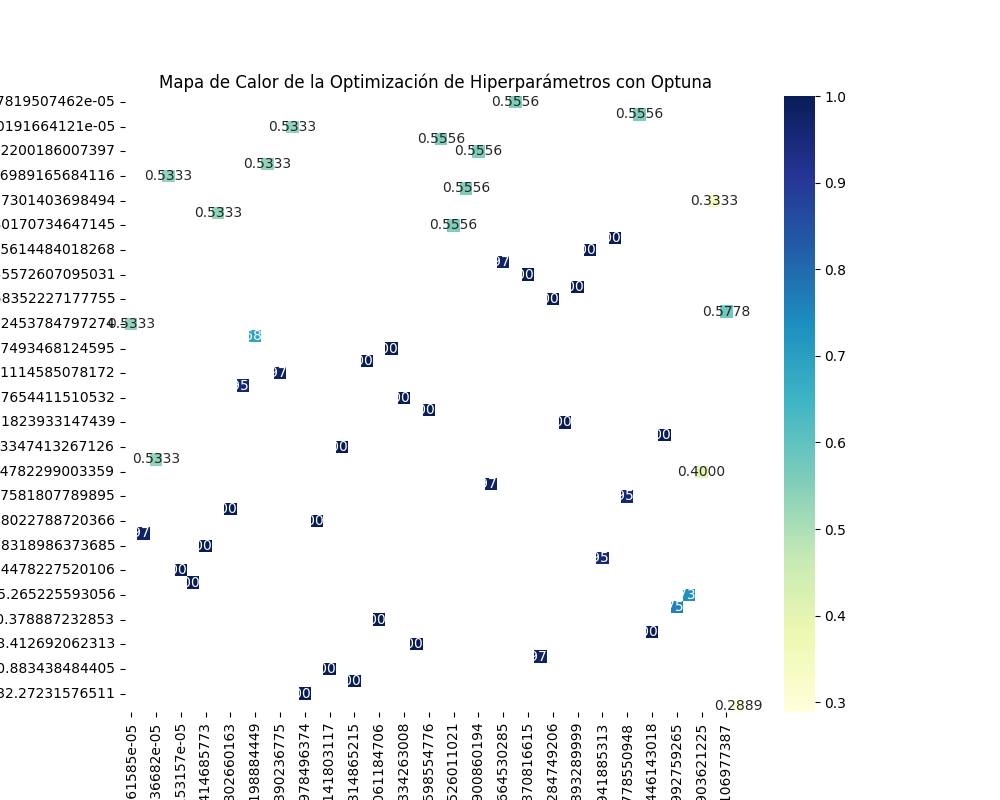
\includegraphics[width=0.8\textwidth]{heatmap_optuna.png}
	\caption{Mapa de calor de la optimización de hiperparámetros con Optuna}
	\label{fig:optuna_heatmap}
\end{figure}

El siguiente código en Python genera el mapa de calor a partir de los resultados de la optimización:

\begin{lstlisting}
	import optuna
	import matplotlib
	import matplotlib.pyplot as plt
	import seaborn as sns
	import numpy as np
	from sklearn.datasets import load_iris
	from sklearn.model_selection import train_test_split
	from sklearn.svm import SVC
	from sklearn.metrics import accuracy_score
	
	# Usar el backend adecuado para evitar el problema de Tkinter
	matplotlib.use('Agg')  # Esto asegura que el gráfico se renderice sin GUI
	
	# Cargar el conjunto de datos Iris
	data = load_iris()
	X = data.data
	y = data.target
	
	# Dividir en entrenamiento y prueba
	X_train, X_test, y_train, y_test = train_test_split(X, y, test_size=0.3, random_state=42)
	
	# Función objetivo para la optimización
	def objective(trial):
	C = trial.suggest_float('C', 1e-5, 1e5, log=True)  # Regularización
	gamma = trial.suggest_float('gamma', 1e-5, 1e5, log=True)  # Parámetro del núcleo RBF
	
	# Crear el modelo con los hiperparámetros sugeridos
	model = SVC(C=C, gamma=gamma)
	model.fit(X_train, y_train)
	
	# Predecir y calcular la precisión
	y_pred = model.predict(X_test)
	accuracy = accuracy_score(y_test, y_pred)
	return accuracy
	
	# Crear el estudio de Optuna
	study = optuna.create_study(direction='maximize')
	
	# Optimizar los hiperparámetros
	study.optimize(objective, n_trials=50)
	
	# Obtener el resultado del estudio
	trials_df = study.trials_dataframe()
	
	# Crear un mapa de calor de los resultados de las pruebas
	# Extraemos solo los hiperparámetros C y gamma
	heatmap_data = trials_df[['params_C', 'params_gamma', 'value']]
	
	# Reestructurar los datos en una matriz para visualización
	heatmap_matrix = heatmap_data.pivot_table(index='params_C', columns='params_gamma', values='value')
	
	# Graficar el mapa de calor
	plt.figure(figsize=(10, 8))
	sns.heatmap(heatmap_matrix, cmap='YlGnBu', annot=True, fmt='.4f')
	plt.title("Mapa de Calor de la Optimización de Hiperparámetros con Optuna")
	plt.xlabel('Gamma')
	plt.ylabel('C')
	
	# Guardar el gráfico en un archivo
	plt.savefig("heatmap_optuna.png")
	
	# Mostrar el gráfico en pantalla
	plt.show()
\end{lstlisting}


\subsection*{Caso de Estudio: Distribución de Infraestructura en Regiones Rurales}
Se puede aplicar GIS para evaluar la distribución de infraestructura pública en áreas rurales. Un análisis típico incluiría:

\begin{itemize}
	\item Identificación de zonas sin acceso a servicios esenciales.
	\item Aplicación de modelos de optimización para proponer nuevas infraestructuras.
	\item Visualización de mapas de calor para determinar áreas con alta demanda de servicios.
\end{itemize}

Este tipo de análisis permite una mejor planificación y distribución de recursos, maximizando el impacto de las inversiones en infraestructura.


\section*{9.4 Aplicaciones del Mundo Real con Censos Peruanos}

\subsection*{Las Aplicaciones Geoespaciales en Perú}
En el Perú, el uso de datos censales combinados con herramientas GIS permite realizar análisis cruciales para la toma de decisiones en planificación urbana, infraestructura, servicios públicos, y políticas sociales. La integración de estos datos facilita la identificación de patrones espaciales que pueden optimizar la distribución de recursos y mejorar la calidad de vida en diferentes regiones del país. Los análisis geoespaciales ayudan a resolver desafíos complejos, como la identificación de áreas desatendidas, la planificación de infraestructura y la mejora de la eficiencia en los servicios públicos. En esta sección, exploramos aplicaciones del análisis geoespacial con censos peruanos en diversas áreas clave.

\subsection*{Optimización de Infraestructura Pública}
El análisis de datos censales y la integración con GIS permite una mejor distribución y accesibilidad de la infraestructura pública, como hospitales, colegios, redes de transporte, agua potable y telecomunicaciones. Esto es fundamental para asegurar que los recursos lleguen a las zonas más necesitadas, especialmente en regiones rurales o marginales. Algunas de las aplicaciones de la optimización de infraestructura incluyen:

\begin{table}[ht]
	\centering
	\caption{Ejemplos de Optimización de Infraestructura Pública}
	\begin{tabularx}{\textwidth}{|l|X|}
		\hline
		\textbf{Aplicación} & \textbf{Descripción} \\
		\hline
		Cobertura de hospitales & Identificar áreas con mayor necesidad de servicios médicos, evaluando la densidad de población y la proximidad a centros de salud. \\
		\hline
		Accesibilidad de escuelas & Determinar la distancia de los centros poblados a los colegios más cercanos, considerando la capacidad de las instituciones y el acceso en transporte. \\
		\hline
		Distribución de redes de telecomunicaciones & Identificar zonas con baja cobertura de internet y telefonía móvil, con el fin de expandir las redes en áreas rurales o alejadas. \\
		\hline
		Red de agua potable y alcantarillado & Evaluar la cobertura de los servicios de agua potable y alcantarillado, identificando zonas con deficiencias en estos servicios esenciales. \\
		\hline
		Energía eléctrica & Analizar la distribución de redes eléctricas y detectar zonas rurales o periurbanas que carecen de acceso a electricidad. \\
		\hline
	\end{tabularx}
	\label{tab:infraestructura}
\end{table}

Además de los ejemplos mencionados, la optimización de infraestructura pública mediante GIS permite planificar la expansión de redes de saneamiento, transporte, y comunicación en zonas rurales, mejorando la accesibilidad y la calidad de vida de las poblaciones más vulnerables.

\subsection*{Modelos Predictivos de Demanda}
El análisis de censos y datos geoespaciales no solo permite optimizar la distribución de recursos en el presente, sino que también puede utilizarse para predecir tendencias futuras en áreas clave. Los modelos predictivos ayudan a anticipar necesidades y planificar la infraestructura antes de que surjan problemas. Algunos ejemplos incluyen:

\begin{itemize}
	\item \textbf{Crecimiento urbano}: Usando los datos de crecimiento poblacional, se pueden desarrollar modelos de expansión urbana para prever el aumento de la población en las ciudades y planificar la expansión de la infraestructura urbana (vivienda, redes de transporte, etc.).
	\item \textbf{Demanda de transporte público}: Predicción del flujo de pasajeros en ciudades como Lima, Arequipa o Trujillo, utilizando datos censales y patrones de movilidad. Esto permite optimizar las rutas de buses y el sistema de metro, así como planificar nuevas líneas de transporte público.
	\item \textbf{Impacto de políticas públicas}: Evaluación del impacto de programas sociales, como los destinados a reducir la pobreza, sobre las diferentes regiones del país. Los datos censales permiten evaluar cómo las políticas afectan a distintos sectores de la población y determinar áreas con mayor necesidad de intervención.
	\item \textbf{Demanda de servicios básicos}: Los datos censales sobre acceso a agua, electricidad, salud y educación pueden predecir la expansión de estos servicios en función del crecimiento poblacional y las necesidades de los diferentes grupos socioeconómicos.
\end{itemize}

Estos modelos predictivos se vuelven fundamentales para planificar con anticipación la infraestructura, de manera que los recursos sean distribuidos de manera eficiente y se maximicen los beneficios a largo plazo.

\subsection*{Caso de Estudio: Planificación de Transporte en Lima Metropolitana}
Un caso concreto de aplicación de datos censales es la planificación del transporte en Lima Metropolitana. A través del análisis de la distribución poblacional y los patrones de movilidad, es posible optimizar las rutas de transporte público y reducir la congestión. El proceso de planificación incluye:

\begin{itemize}
	\item Obtención de datos del censo de población y movilidad urbana, lo que permite conocer los flujos de pasajeros, puntos de congestión y necesidades de transporte en diferentes distritos de Lima.
	\item Identificación de áreas con mayor demanda de transporte, como aquellas con alta concentración de población, áreas industriales o comerciales, y escaso acceso a sistemas de transporte público.
	\item Simulación de rutas óptimas para reducir la congestión y los tiempos de viaje. Utilizando algoritmos de optimización, se pueden diseñar rutas de transporte eficientes que conecten las principales zonas de la ciudad.
	\item Implementación de mapas de calor para visualizar la demanda de transporte en diferentes zonas de la ciudad, ayudando a priorizar las inversiones en infraestructura de transporte público.
\end{itemize}

Estos análisis son fundamentales para reducir la congestión vehicular, mejorar la calidad del aire y optimizar los tiempos de desplazamiento de los ciudadanos.

\subsection*{Uso de Mapas de Calor para Identificación de Zonas Críticas}
Los mapas de calor son herramientas poderosas para visualizar patrones espaciales de interés, ya que permiten identificar áreas con características similares y tomar decisiones basadas en datos concretos. Algunas aplicaciones clave incluyen:

\begin{itemize}
	\item \textbf{Desigualdad socioeconómica}: Utilizando datos de pobreza y acceso a servicios, se pueden generar mapas de calor para identificar las regiones más vulnerables y priorizar la implementación de programas de asistencia social y servicios básicos.
	\item \textbf{Áreas con mayor demanda de servicios públicos}: Utilizando el Directorio Nacional de Centros Poblados 2023 y los datos del censo, se pueden generar mapas de calor que permitan visualizar la cobertura de servicios de salud, educación, agua potable, electricidad, entre otros, y planificar la expansión de estos servicios en zonas desatendidas.
	\item \textbf{Análisis de movilidad y transporte}: Evaluar la accesibilidad a estaciones de transporte, como paraderos de buses, estaciones de metro o terminales de tren, y optimizar la distribución de rutas. Los mapas de calor muestran los puntos de mayor aglomeración y permiten planificar nuevas rutas de transporte público.
	\item \textbf{Seguridad ciudadana}: Los mapas de calor también se utilizan para analizar la incidencia de delitos y generar estrategias para la mejora de la seguridad en las áreas más afectadas. Esto facilita la asignación de recursos a la prevención del crimen y la respuesta a emergencias.
	\item \textbf{Acceso a servicios de emergencia}: Se pueden crear mapas de calor para evaluar los tiempos de respuesta de ambulancias y vehículos de emergencia, ayudando a identificar áreas que necesitan mejorar el acceso a servicios de salud de emergencia.
\end{itemize}

El uso de mapas de calor permite a los planificadores ver patrones espaciales de manera clara y efectiva, facilitando la toma de decisiones informadas para mejorar la infraestructura y los servicios públicos en el país.

\subsection*{Ejemplo de Implementación: Generación de Mapas de Calor en Python}
A continuación, se presenta un ejemplo de cómo generar un mapa de calor utilizando datos de optimización de infraestructura, como la ubicación de centros poblados y su acceso a servicios esenciales. Este ejemplo usa **Optuna** para optimizar los parámetros de ubicación y **Seaborn** para crear el gráfico:

\begin{lstlisting}
	import optuna
	import matplotlib.pyplot as plt
	import seaborn as sns
	
	# Ejemplo de datos (centrado en infraestructura)
	heatmap_data = {
		'Zona': ['Norte', 'Sur', 'Este', 'Oeste'],
		'Acceso a Salud': [0.75, 0.50, 0.80, 0.65],
		'Acceso a Educación': [0.60, 0.55, 0.75, 0.45],
		'Acceso a Transporte': [0.80, 0.60, 0.70, 0.90]
	}
	
	# Convertir a DataFrame
	import pandas as pd
	df = pd.DataFrame(heatmap_data)
	
	# Crear mapa de calor
	plt.figure(figsize=(10, 6))
	sns.heatmap(df.set_index('Zona'), annot=True, cmap='YlGnBu', fmt='.2f')
	
	# Título y etiquetas
	plt.title('Mapa de Calor: Acceso a Servicios en Zonas de Lima Metropolitana')
	plt.ylabel('Zonas')
	plt.xlabel('Servicios')
	
	# Mostrar el gráfico
	plt.show()
\end{lstlisting}

\begin{thebibliography}{9}
	
	\bibitem{inei_censo} 
	Instituto Nacional de Estadística e Informática (INEI). (2017). \textit{Censo Nacional de Población y Vivienda}. Recuperado de: \url{https://www.inei.gob.pe}
	
	\bibitem{inei_centros_poblados} 
	Instituto Nacional de Estadística e Informática (INEI). (2023). \textit{Directorio Nacional de Centros Poblados}. Recuperado de: \url{https://www.inei.gob.pe}
	
	\bibitem{qgis_doc} 
	QGIS Documentation Team. (2024). \textit{QGIS User Guide}. Recuperado de: \url{https://qgis.org/en/docs/index.html}
	
	\bibitem{geopandas} 
	Kelsey Jordahl et al. (2024). \textit{GeoPandas: Geographic data in Python}. Recuperado de: \url{https://geopandas.org}
	
	
	\bibitem{transport_model} 
	Rodrigue, J.-P., Comtois, C., & Slack, B. (2017). \textit{The Geography of Transport Systems}. Routledge.
	
	\bibitem{urban_planning} 
	Batty, M. (2013). \textit{The New Science of Cities}. MIT Press.
	
	\bibitem{arcgis_doc} 
	Esri. (2024). \textit{ArcGIS Documentation}. Recuperado de: \url{https://desktop.arcgis.com/en/documentation/}
	
\end{thebibliography}

\end{document}
